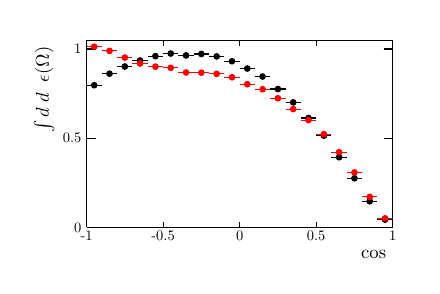
\begin{tikzpicture}
\pgfdeclareplotmark{cross} {
\pgfpathmoveto{\pgfpoint{-0.3\pgfplotmarksize}{\pgfplotmarksize}}
\pgfpathlineto{\pgfpoint{+0.3\pgfplotmarksize}{\pgfplotmarksize}}
\pgfpathlineto{\pgfpoint{+0.3\pgfplotmarksize}{0.3\pgfplotmarksize}}
\pgfpathlineto{\pgfpoint{+1\pgfplotmarksize}{0.3\pgfplotmarksize}}
\pgfpathlineto{\pgfpoint{+1\pgfplotmarksize}{-0.3\pgfplotmarksize}}
\pgfpathlineto{\pgfpoint{+0.3\pgfplotmarksize}{-0.3\pgfplotmarksize}}
\pgfpathlineto{\pgfpoint{+0.3\pgfplotmarksize}{-1.\pgfplotmarksize}}
\pgfpathlineto{\pgfpoint{-0.3\pgfplotmarksize}{-1.\pgfplotmarksize}}
\pgfpathlineto{\pgfpoint{-0.3\pgfplotmarksize}{-0.3\pgfplotmarksize}}
\pgfpathlineto{\pgfpoint{-1.\pgfplotmarksize}{-0.3\pgfplotmarksize}}
\pgfpathlineto{\pgfpoint{-1.\pgfplotmarksize}{0.3\pgfplotmarksize}}
\pgfpathlineto{\pgfpoint{-0.3\pgfplotmarksize}{0.3\pgfplotmarksize}}
\pgfpathclose
\pgfusepathqstroke
}
\pgfdeclareplotmark{cross*} {
\pgfpathmoveto{\pgfpoint{-0.3\pgfplotmarksize}{\pgfplotmarksize}}
\pgfpathlineto{\pgfpoint{+0.3\pgfplotmarksize}{\pgfplotmarksize}}
\pgfpathlineto{\pgfpoint{+0.3\pgfplotmarksize}{0.3\pgfplotmarksize}}
\pgfpathlineto{\pgfpoint{+1\pgfplotmarksize}{0.3\pgfplotmarksize}}
\pgfpathlineto{\pgfpoint{+1\pgfplotmarksize}{-0.3\pgfplotmarksize}}
\pgfpathlineto{\pgfpoint{+0.3\pgfplotmarksize}{-0.3\pgfplotmarksize}}
\pgfpathlineto{\pgfpoint{+0.3\pgfplotmarksize}{-1.\pgfplotmarksize}}
\pgfpathlineto{\pgfpoint{-0.3\pgfplotmarksize}{-1.\pgfplotmarksize}}
\pgfpathlineto{\pgfpoint{-0.3\pgfplotmarksize}{-0.3\pgfplotmarksize}}
\pgfpathlineto{\pgfpoint{-1.\pgfplotmarksize}{-0.3\pgfplotmarksize}}
\pgfpathlineto{\pgfpoint{-1.\pgfplotmarksize}{0.3\pgfplotmarksize}}
\pgfpathlineto{\pgfpoint{-0.3\pgfplotmarksize}{0.3\pgfplotmarksize}}
\pgfpathclose
\pgfusepathqfillstroke
}
\pgfdeclareplotmark{newstar} {
\pgfpathmoveto{\pgfqpoint{0pt}{\pgfplotmarksize}}
\pgfpathlineto{\pgfqpointpolar{44}{0.5\pgfplotmarksize}}
\pgfpathlineto{\pgfqpointpolar{18}{\pgfplotmarksize}}
\pgfpathlineto{\pgfqpointpolar{-20}{0.5\pgfplotmarksize}}
\pgfpathlineto{\pgfqpointpolar{-54}{\pgfplotmarksize}}
\pgfpathlineto{\pgfqpointpolar{-90}{0.5\pgfplotmarksize}}
\pgfpathlineto{\pgfqpointpolar{234}{\pgfplotmarksize}}
\pgfpathlineto{\pgfqpointpolar{198}{0.5\pgfplotmarksize}}
\pgfpathlineto{\pgfqpointpolar{162}{\pgfplotmarksize}}
\pgfpathlineto{\pgfqpointpolar{134}{0.5\pgfplotmarksize}}
\pgfpathclose
\pgfusepathqstroke
}
\pgfdeclareplotmark{newstar*} {
\pgfpathmoveto{\pgfqpoint{0pt}{\pgfplotmarksize}}
\pgfpathlineto{\pgfqpointpolar{44}{0.5\pgfplotmarksize}}
\pgfpathlineto{\pgfqpointpolar{18}{\pgfplotmarksize}}
\pgfpathlineto{\pgfqpointpolar{-20}{0.5\pgfplotmarksize}}
\pgfpathlineto{\pgfqpointpolar{-54}{\pgfplotmarksize}}
\pgfpathlineto{\pgfqpointpolar{-90}{0.5\pgfplotmarksize}}
\pgfpathlineto{\pgfqpointpolar{234}{\pgfplotmarksize}}
\pgfpathlineto{\pgfqpointpolar{198}{0.5\pgfplotmarksize}}
\pgfpathlineto{\pgfqpointpolar{162}{\pgfplotmarksize}}
\pgfpathlineto{\pgfqpointpolar{134}{0.5\pgfplotmarksize}}
\pgfpathclose
\pgfusepathqfillstroke
}
\definecolor{c}{rgb}{1,1,1};
\draw [color=c, fill=c] (0.1,3.20034) rectangle (4.9,6.21242);
\draw [color=c, fill=c] (0.772,3.68227) rectangle (4.66,6.06181);
\definecolor{c}{rgb}{0,0,0};
\draw [c] (0.772,3.68227) -- (0.772,6.06181) -- (4.66,6.06181) -- (4.66,3.68227) -- (0.772,3.68227);
\draw [c,line width=0.4] (0.8692,5.47816) -- (0.8692,5.48875);
\draw [c,line width=0.4] (0.8692,5.48875) -- (0.8692,5.49933);
\draw [c,line width=0.4] (0.772,5.48875) -- (0.8692,5.48875);
\draw [c,line width=0.4] (0.8692,5.48875) -- (0.9664,5.48875);
\foreach \P in {(0.8692,5.48875)}{\draw[mark options={color=c,fill=c},mark size=2.402402pt,mark=*,mark size=1pt] plot coordinates {\P};}
\draw [c,line width=0.4] (1.0636,5.62474) -- (1.0636,5.63481);
\draw [c,line width=0.4] (1.0636,5.63481) -- (1.0636,5.64489);
\draw [c,line width=0.4] (0.9664,5.63481) -- (1.0636,5.63481);
\draw [c,line width=0.4] (1.0636,5.63481) -- (1.1608,5.63481);
\foreach \P in {(1.0636,5.63481)}{\draw[mark options={color=c,fill=c},mark size=2.402402pt,mark=*,mark size=1pt] plot coordinates {\P};}
\draw [c,line width=0.4] (1.258,5.7159) -- (1.258,5.72607);
\draw [c,line width=0.4] (1.258,5.72607) -- (1.258,5.73625);
\draw [c,line width=0.4] (1.1608,5.72607) -- (1.258,5.72607);
\draw [c,line width=0.4] (1.258,5.72607) -- (1.3552,5.72607);
\foreach \P in {(1.258,5.72607)}{\draw[mark options={color=c,fill=c},mark size=2.402402pt,mark=*,mark size=1pt] plot coordinates {\P};}
\draw [c,line width=0.4] (1.4524,5.79234) -- (1.4524,5.8029);
\draw [c,line width=0.4] (1.4524,5.8029) -- (1.4524,5.81346);
\draw [c,line width=0.4] (1.3552,5.8029) -- (1.4524,5.8029);
\draw [c,line width=0.4] (1.4524,5.8029) -- (1.5496,5.8029);
\foreach \P in {(1.4524,5.8029)}{\draw[mark options={color=c,fill=c},mark size=2.402402pt,mark=*,mark size=1pt] plot coordinates {\P};}
\draw [c,line width=0.4] (1.6468,5.847) -- (1.6468,5.85792);
\draw [c,line width=0.4] (1.6468,5.85792) -- (1.6468,5.86884);
\draw [c,line width=0.4] (1.5496,5.85792) -- (1.6468,5.85792);
\draw [c,line width=0.4] (1.6468,5.85792) -- (1.744,5.85792);
\foreach \P in {(1.6468,5.85792)}{\draw[mark options={color=c,fill=c},mark size=2.402402pt,mark=*,mark size=1pt] plot coordinates {\P};}
\draw [c,line width=0.4] (1.8412,5.8798) -- (1.8412,5.89116);
\draw [c,line width=0.4] (1.8412,5.89116) -- (1.8412,5.90251);
\draw [c,line width=0.4] (1.744,5.89116) -- (1.8412,5.89116);
\draw [c,line width=0.4] (1.8412,5.89116) -- (1.9384,5.89116);
\foreach \P in {(1.8412,5.89116)}{\draw[mark options={color=c,fill=c},mark size=2.402402pt,mark=*,mark size=1pt] plot coordinates {\P};}
\draw [c,line width=0.4] (2.0356,5.85532) -- (2.0356,5.86694);
\draw [c,line width=0.4] (2.0356,5.86694) -- (2.0356,5.87856);
\draw [c,line width=0.4] (1.9384,5.86694) -- (2.0356,5.86694);
\draw [c,line width=0.4] (2.0356,5.86694) -- (2.1328,5.86694);
\foreach \P in {(2.0356,5.86694)}{\draw[mark options={color=c,fill=c},mark size=2.402402pt,mark=*,mark size=1pt] plot coordinates {\P};}
\draw [c,line width=0.4] (2.23,5.87314) -- (2.23,5.88515);
\draw [c,line width=0.4] (2.23,5.88515) -- (2.23,5.89716);
\draw [c,line width=0.4] (2.1328,5.88515) -- (2.23,5.88515);
\draw [c,line width=0.4] (2.23,5.88515) -- (2.3272,5.88515);
\foreach \P in {(2.23,5.88515)}{\draw[mark options={color=c,fill=c},mark size=2.402402pt,mark=*,mark size=1pt] plot coordinates {\P};}
\draw [c,line width=0.4] (2.4244,5.84239) -- (2.4244,5.85463);
\draw [c,line width=0.4] (2.4244,5.85463) -- (2.4244,5.86686);
\draw [c,line width=0.4] (2.3272,5.85463) -- (2.4244,5.85463);
\draw [c,line width=0.4] (2.4244,5.85463) -- (2.5216,5.85463);
\foreach \P in {(2.4244,5.85463)}{\draw[mark options={color=c,fill=c},mark size=2.402402pt,mark=*,mark size=1pt] plot coordinates {\P};}
\draw [c,line width=0.4] (2.6188,5.78114) -- (2.6188,5.79337);
\draw [c,line width=0.4] (2.6188,5.79337) -- (2.6188,5.8056);
\draw [c,line width=0.4] (2.5216,5.79337) -- (2.6188,5.79337);
\draw [c,line width=0.4] (2.6188,5.79337) -- (2.716,5.79337);
\foreach \P in {(2.6188,5.79337)}{\draw[mark options={color=c,fill=c},mark size=2.402402pt,mark=*,mark size=1pt] plot coordinates {\P};}
\draw [c,line width=0.4] (2.8132,5.68836) -- (2.8132,5.70028);
\draw [c,line width=0.4] (2.8132,5.70028) -- (2.8132,5.71221);
\draw [c,line width=0.4] (2.716,5.70028) -- (2.8132,5.70028);
\draw [c,line width=0.4] (2.8132,5.70028) -- (2.9104,5.70028);
\foreach \P in {(2.8132,5.70028)}{\draw[mark options={color=c,fill=c},mark size=2.402402pt,mark=*,mark size=1pt] plot coordinates {\P};}
\draw [c,line width=0.4] (3.0076,5.58717) -- (3.0076,5.59864);
\draw [c,line width=0.4] (3.0076,5.59864) -- (3.0076,5.61011);
\draw [c,line width=0.4] (2.9104,5.59864) -- (3.0076,5.59864);
\draw [c,line width=0.4] (3.0076,5.59864) -- (3.1048,5.59864);
\foreach \P in {(3.0076,5.59864)}{\draw[mark options={color=c,fill=c},mark size=2.402402pt,mark=*,mark size=1pt] plot coordinates {\P};}
\draw [c,line width=0.4] (3.202,5.42933) -- (3.202,5.44001);
\draw [c,line width=0.4] (3.202,5.44001) -- (3.202,5.45069);
\draw [c,line width=0.4] (3.1048,5.44001) -- (3.202,5.44001);
\draw [c,line width=0.4] (3.202,5.44001) -- (3.2992,5.44001);
\foreach \P in {(3.202,5.44001)}{\draw[mark options={color=c,fill=c},mark size=2.402402pt,mark=*,mark size=1pt] plot coordinates {\P};}
\draw [c,line width=0.4] (3.3964,5.26048) -- (3.3964,5.27032);
\draw [c,line width=0.4] (3.3964,5.27032) -- (3.3964,5.28016);
\draw [c,line width=0.4] (3.2992,5.27032) -- (3.3964,5.27032);
\draw [c,line width=0.4] (3.3964,5.27032) -- (3.4936,5.27032);
\foreach \P in {(3.3964,5.27032)}{\draw[mark options={color=c,fill=c},mark size=2.402402pt,mark=*,mark size=1pt] plot coordinates {\P};}
\draw [c,line width=0.4] (3.5908,5.0633) -- (3.5908,5.0722);
\draw [c,line width=0.4] (3.5908,5.0722) -- (3.5908,5.0811);
\draw [c,line width=0.4] (3.4936,5.0722) -- (3.5908,5.0722);
\draw [c,line width=0.4] (3.5908,5.0722) -- (3.688,5.0722);
\foreach \P in {(3.5908,5.0722)}{\draw[mark options={color=c,fill=c},mark size=2.402402pt,mark=*,mark size=1pt] plot coordinates {\P};}
\draw [c,line width=0.4] (3.7852,4.84046) -- (3.7852,4.84837);
\draw [c,line width=0.4] (3.7852,4.84837) -- (3.7852,4.85628);
\draw [c,line width=0.4] (3.688,4.84837) -- (3.7852,4.84837);
\draw [c,line width=0.4] (3.7852,4.84837) -- (3.8824,4.84837);
\foreach \P in {(3.7852,4.84837)}{\draw[mark options={color=c,fill=c},mark size=2.402402pt,mark=*,mark size=1pt] plot coordinates {\P};}
\draw [c,line width=0.4] (3.9796,4.56728) -- (3.9796,4.57401);
\draw [c,line width=0.4] (3.9796,4.57401) -- (3.9796,4.58074);
\draw [c,line width=0.4] (3.8824,4.57401) -- (3.9796,4.57401);
\draw [c,line width=0.4] (3.9796,4.57401) -- (4.0768,4.57401);
\foreach \P in {(3.9796,4.57401)}{\draw[mark options={color=c,fill=c},mark size=2.402402pt,mark=*,mark size=1pt] plot coordinates {\P};}
\draw [c,line width=0.4] (4.174,4.30147) -- (4.174,4.30707);
\draw [c,line width=0.4] (4.174,4.30707) -- (4.174,4.31267);
\draw [c,line width=0.4] (4.0768,4.30707) -- (4.174,4.30707);
\draw [c,line width=0.4] (4.174,4.30707) -- (4.2712,4.30707);
\foreach \P in {(4.174,4.30707)}{\draw[mark options={color=c,fill=c},mark size=2.402402pt,mark=*,mark size=1pt] plot coordinates {\P};}
\draw [c,line width=0.4] (4.3684,4.01049) -- (4.3684,4.01452);
\draw [c,line width=0.4] (4.3684,4.01452) -- (4.3684,4.01856);
\draw [c,line width=0.4] (4.2712,4.01452) -- (4.3684,4.01452);
\draw [c,line width=0.4] (4.3684,4.01452) -- (4.4656,4.01452);
\foreach \P in {(4.3684,4.01452)}{\draw[mark options={color=c,fill=c},mark size=2.402402pt,mark=*,mark size=1pt] plot coordinates {\P};}
\draw [c,line width=0.4] (4.5628,3.7793) -- (4.5628,3.78155);
\draw [c,line width=0.4] (4.5628,3.78155) -- (4.5628,3.7838);
\draw [c,line width=0.4] (4.4656,3.78155) -- (4.5628,3.78155);
\draw [c,line width=0.4] (4.5628,3.78155) -- (4.66,3.78155);
\foreach \P in {(4.5628,3.78155)}{\draw[mark options={color=c,fill=c},mark size=2.402402pt,mark=*,mark size=1pt] plot coordinates {\P};}
\draw [c,line width=0.4] (0.772,3.68227) -- (4.66,3.68227);
\draw [anchor= east] (4.66,3.34492) node[scale=0.672711, rotate=0]{$\cos\thetaK$};
\draw [c,line width=0.4] (0.772,3.75546) -- (0.772,3.68227);
\draw [c,line width=0.4] (1.744,3.75546) -- (1.744,3.68227);
\draw [c,line width=0.4] (2.716,3.75546) -- (2.716,3.68227);
\draw [c,line width=0.4] (3.688,3.75546) -- (3.688,3.68227);
\draw [c,line width=0.4] (4.66,3.75546) -- (4.66,3.68227);
\draw [anchor=base] (0.772,3.51962) node[scale=0.52322, rotate=0]{-1};
\draw [anchor=base] (1.744,3.51962) node[scale=0.52322, rotate=0]{-0.5};
\draw [anchor=base] (2.716,3.51962) node[scale=0.52322, rotate=0]{0};
\draw [anchor=base] (3.688,3.51962) node[scale=0.52322, rotate=0]{0.5};
\draw [anchor=base] (4.66,3.51962) node[scale=0.52322, rotate=0]{1};
\draw [c,line width=0.4] (0.772,6.06181) -- (4.66,6.06181);
\draw [c,line width=0.4] (0.772,5.98862) -- (0.772,6.06181);
\draw [c,line width=0.4] (1.744,5.98862) -- (1.744,6.06181);
\draw [c,line width=0.4] (2.716,5.98862) -- (2.716,6.06181);
\draw [c,line width=0.4] (3.688,5.98862) -- (3.688,6.06181);
\draw [c,line width=0.4] (4.66,5.98862) -- (4.66,6.06181);
\draw [c,line width=0.4] (0.772,3.68227) -- (0.772,6.06181);
\draw [anchor= east] (0.2344,6.06181) node[scale=0.672711, rotate=90]{$\int d\thetamu \; d\phihel \;\; \epsilon(\Omega) $};
\draw [c,line width=0.4] (0.88576,3.68227) -- (0.772,3.68227);
\draw [c,line width=0.4] (0.88576,4.81538) -- (0.772,4.81538);
\draw [c,line width=0.4] (0.88576,5.9485) -- (0.772,5.9485);
\draw [c,line width=0.4] (0.88576,5.9485) -- (0.772,5.9485);
\draw [anchor= east] (0.772,3.68227) node[scale=0.52322, rotate=0]{0};
\draw [anchor= east] (0.772,4.81538) node[scale=0.52322, rotate=0]{0.5};
\draw [anchor= east] (0.772,5.9485) node[scale=0.52322, rotate=0]{1};
\draw [c,line width=0.4] (4.66,3.68227) -- (4.66,6.06181);
\draw [c,line width=0.4] (4.54624,3.68227) -- (4.66,3.68227);
\draw [c,line width=0.4] (4.54624,4.81538) -- (4.66,4.81538);
\draw [c,line width=0.4] (4.54624,5.9485) -- (4.66,5.9485);
\draw [c,line width=0.4] (4.54624,5.9485) -- (4.66,5.9485);
\definecolor{c}{rgb}{1,0,0};
\draw [c,line width=0.4] (0.8692,5.94933) -- (0.8692,5.97743);
\draw [c,line width=0.4] (0.8692,5.97743) -- (0.8692,6.00552);
\draw [c,line width=0.4] (0.772,5.97743) -- (0.8692,5.97743);
\draw [c,line width=0.4] (0.8692,5.97743) -- (0.9664,5.97743);
\foreach \P in {(0.8692,5.97743)}{\draw[mark options={color=c,fill=c},mark size=2.402402pt,mark=*,mark size=1pt] plot coordinates {\P};}
\draw [c,line width=0.4] (1.0636,5.90049) -- (1.0636,5.92445);
\draw [c,line width=0.4] (1.0636,5.92445) -- (1.0636,5.94841);
\draw [c,line width=0.4] (0.9664,5.92445) -- (1.0636,5.92445);
\draw [c,line width=0.4] (1.0636,5.92445) -- (1.1608,5.92445);
\foreach \P in {(1.0636,5.92445)}{\draw[mark options={color=c,fill=c},mark size=2.402402pt,mark=*,mark size=1pt] plot coordinates {\P};}
\draw [c,line width=0.4] (1.258,5.82086) -- (1.258,5.83997);
\draw [c,line width=0.4] (1.258,5.83997) -- (1.258,5.85907);
\draw [c,line width=0.4] (1.1608,5.83997) -- (1.258,5.83997);
\draw [c,line width=0.4] (1.258,5.83997) -- (1.3552,5.83997);
\foreach \P in {(1.258,5.83997)}{\draw[mark options={color=c,fill=c},mark size=2.402402pt,mark=*,mark size=1pt] plot coordinates {\P};}
\draw [c,line width=0.4] (1.4524,5.7479) -- (1.4524,5.76464);
\draw [c,line width=0.4] (1.4524,5.76464) -- (1.4524,5.78138);
\draw [c,line width=0.4] (1.3552,5.76464) -- (1.4524,5.76464);
\draw [c,line width=0.4] (1.4524,5.76464) -- (1.5496,5.76464);
\foreach \P in {(1.4524,5.76464)}{\draw[mark options={color=c,fill=c},mark size=2.402402pt,mark=*,mark size=1pt] plot coordinates {\P};}
\draw [c,line width=0.4] (1.6468,5.70986) -- (1.6468,5.7247);
\draw [c,line width=0.4] (1.6468,5.7247) -- (1.6468,5.73954);
\draw [c,line width=0.4] (1.5496,5.7247) -- (1.6468,5.7247);
\draw [c,line width=0.4] (1.6468,5.7247) -- (1.744,5.7247);
\foreach \P in {(1.6468,5.7247)}{\draw[mark options={color=c,fill=c},mark size=2.402402pt,mark=*,mark size=1pt] plot coordinates {\P};}
\draw [c,line width=0.4] (1.8412,5.69479) -- (1.8412,5.70939);
\draw [c,line width=0.4] (1.8412,5.70939) -- (1.8412,5.72399);
\draw [c,line width=0.4] (1.744,5.70939) -- (1.8412,5.70939);
\draw [c,line width=0.4] (1.8412,5.70939) -- (1.9384,5.70939);
\foreach \P in {(1.8412,5.70939)}{\draw[mark options={color=c,fill=c},mark size=2.402402pt,mark=*,mark size=1pt] plot coordinates {\P};}
\draw [c,line width=0.4] (2.0356,5.63623) -- (2.0356,5.6501);
\draw [c,line width=0.4] (2.0356,5.6501) -- (2.0356,5.66398);
\draw [c,line width=0.4] (1.9384,5.6501) -- (2.0356,5.6501);
\draw [c,line width=0.4] (2.0356,5.6501) -- (2.1328,5.6501);
\foreach \P in {(2.0356,5.6501)}{\draw[mark options={color=c,fill=c},mark size=2.402402pt,mark=*,mark size=1pt] plot coordinates {\P};}
\draw [c,line width=0.4] (2.23,5.63426) -- (2.23,5.64795);
\draw [c,line width=0.4] (2.23,5.64795) -- (2.23,5.66165);
\draw [c,line width=0.4] (2.1328,5.64795) -- (2.23,5.64795);
\draw [c,line width=0.4] (2.23,5.64795) -- (2.3272,5.64795);
\foreach \P in {(2.23,5.64795)}{\draw[mark options={color=c,fill=c},mark size=2.402402pt,mark=*,mark size=1pt] plot coordinates {\P};}
\draw [c,line width=0.4] (2.4244,5.61851) -- (2.4244,5.63271);
\draw [c,line width=0.4] (2.4244,5.63271) -- (2.4244,5.6469);
\draw [c,line width=0.4] (2.3272,5.63271) -- (2.4244,5.63271);
\draw [c,line width=0.4] (2.4244,5.63271) -- (2.5216,5.63271);
\foreach \P in {(2.4244,5.63271)}{\draw[mark options={color=c,fill=c},mark size=2.402402pt,mark=*,mark size=1pt] plot coordinates {\P};}
\draw [c,line width=0.4] (2.6188,5.57535) -- (2.6188,5.5894);
\draw [c,line width=0.4] (2.6188,5.5894) -- (2.6188,5.60346);
\draw [c,line width=0.4] (2.5216,5.5894) -- (2.6188,5.5894);
\draw [c,line width=0.4] (2.6188,5.5894) -- (2.716,5.5894);
\foreach \P in {(2.6188,5.5894)}{\draw[mark options={color=c,fill=c},mark size=2.402402pt,mark=*,mark size=1pt] plot coordinates {\P};}
\draw [c,line width=0.4] (2.8132,5.48802) -- (2.8132,5.50127);
\draw [c,line width=0.4] (2.8132,5.50127) -- (2.8132,5.51452);
\draw [c,line width=0.4] (2.716,5.50127) -- (2.8132,5.50127);
\draw [c,line width=0.4] (2.8132,5.50127) -- (2.9104,5.50127);
\foreach \P in {(2.8132,5.50127)}{\draw[mark options={color=c,fill=c},mark size=2.402402pt,mark=*,mark size=1pt] plot coordinates {\P};}
\draw [c,line width=0.4] (3.0076,5.42383) -- (3.0076,5.43753);
\draw [c,line width=0.4] (3.0076,5.43753) -- (3.0076,5.45123);
\draw [c,line width=0.4] (2.9104,5.43753) -- (3.0076,5.43753);
\draw [c,line width=0.4] (3.0076,5.43753) -- (3.1048,5.43753);
\foreach \P in {(3.0076,5.43753)}{\draw[mark options={color=c,fill=c},mark size=2.402402pt,mark=*,mark size=1pt] plot coordinates {\P};}
\draw [c,line width=0.4] (3.202,5.3098) -- (3.202,5.32344);
\draw [c,line width=0.4] (3.202,5.32344) -- (3.202,5.33709);
\draw [c,line width=0.4] (3.1048,5.32344) -- (3.202,5.32344);
\draw [c,line width=0.4] (3.202,5.32344) -- (3.2992,5.32344);
\foreach \P in {(3.202,5.32344)}{\draw[mark options={color=c,fill=c},mark size=2.402402pt,mark=*,mark size=1pt] plot coordinates {\P};}
\draw [c,line width=0.4] (3.3964,5.17167) -- (3.3964,5.18578);
\draw [c,line width=0.4] (3.3964,5.18578) -- (3.3964,5.19989);
\draw [c,line width=0.4] (3.2992,5.18578) -- (3.3964,5.18578);
\draw [c,line width=0.4] (3.3964,5.18578) -- (3.4936,5.18578);
\foreach \P in {(3.3964,5.18578)}{\draw[mark options={color=c,fill=c},mark size=2.402402pt,mark=*,mark size=1pt] plot coordinates {\P};}
\draw [c,line width=0.4] (3.5908,5.03178) -- (3.5908,5.04591);
\draw [c,line width=0.4] (3.5908,5.04591) -- (3.5908,5.06003);
\draw [c,line width=0.4] (3.4936,5.04591) -- (3.5908,5.04591);
\draw [c,line width=0.4] (3.5908,5.04591) -- (3.688,5.04591);
\foreach \P in {(3.5908,5.04591)}{\draw[mark options={color=c,fill=c},mark size=2.402402pt,mark=*,mark size=1pt] plot coordinates {\P};}
\draw [c,line width=0.4] (3.7852,4.85344) -- (3.7852,4.86764);
\draw [c,line width=0.4] (3.7852,4.86764) -- (3.7852,4.88184);
\draw [c,line width=0.4] (3.688,4.86764) -- (3.7852,4.86764);
\draw [c,line width=0.4] (3.7852,4.86764) -- (3.8824,4.86764);
\foreach \P in {(3.7852,4.86764)}{\draw[mark options={color=c,fill=c},mark size=2.402402pt,mark=*,mark size=1pt] plot coordinates {\P};}
\draw [c,line width=0.4] (3.9796,4.6233) -- (3.9796,4.63823);
\draw [c,line width=0.4] (3.9796,4.63823) -- (3.9796,4.65316);
\draw [c,line width=0.4] (3.8824,4.63823) -- (3.9796,4.63823);
\draw [c,line width=0.4] (3.9796,4.63823) -- (4.0768,4.63823);
\foreach \P in {(3.9796,4.63823)}{\draw[mark options={color=c,fill=c},mark size=2.402402pt,mark=*,mark size=1pt] plot coordinates {\P};}
\draw [c,line width=0.4] (4.174,4.36947) -- (4.174,4.38139);
\draw [c,line width=0.4] (4.174,4.38139) -- (4.174,4.39332);
\draw [c,line width=0.4] (4.0768,4.38139) -- (4.174,4.38139);
\draw [c,line width=0.4] (4.174,4.38139) -- (4.2712,4.38139);
\foreach \P in {(4.174,4.38139)}{\draw[mark options={color=c,fill=c},mark size=2.402402pt,mark=*,mark size=1pt] plot coordinates {\P};}
\draw [c,line width=0.4] (4.3684,4.0611) -- (4.3684,4.07059);
\draw [c,line width=0.4] (4.3684,4.07059) -- (4.3684,4.08008);
\draw [c,line width=0.4] (4.2712,4.07059) -- (4.3684,4.07059);
\draw [c,line width=0.4] (4.3684,4.07059) -- (4.4656,4.07059);
\foreach \P in {(4.3684,4.07059)}{\draw[mark options={color=c,fill=c},mark size=2.402402pt,mark=*,mark size=1pt] plot coordinates {\P};}
\draw [c,line width=0.4] (4.5628,3.79304) -- (4.5628,3.79775);
\draw [c,line width=0.4] (4.5628,3.79775) -- (4.5628,3.80247);
\draw [c,line width=0.4] (4.4656,3.79775) -- (4.5628,3.79775);
\draw [c,line width=0.4] (4.5628,3.79775) -- (4.66,3.79775);
\foreach \P in {(4.5628,3.79775)}{\draw[mark options={color=c,fill=c},mark size=2.402402pt,mark=*,mark size=1pt] plot coordinates {\P};}
\end{tikzpicture}
